\ifdefined\pdfobjcompresslevel
  \pdfobjcompresslevel=0
\fi
\documentclass[runningheads]{llncs}

\usepackage{cmap}
\usepackage[T1]{fontenc}
\usepackage{lmodern}
\usepackage{graphicx}
\usepackage{booktabs}
\usepackage{xspace}
\usepackage{array}
\usepackage{multirow}
\usepackage{xcolor}
\usepackage{amsmath}
\usepackage[hidelinks]{hyperref}
\makeatletter
\def\UrlOrds{\do\*\do\~\do\'\do\"\do\:}%
\def\UrlBreaks{\do\/\do\.\do\-}
\def\UrlBigBreaks{\do@url@hyp}
\makeatother
\usepackage{placeins}
\usepackage{tikz}
\usetikzlibrary{arrows.meta,positioning,shapes.geometric,fit,backgrounds,shadows,calc}
\usepackage{orcidlink}
\renewcommand{\orcidID}[1]{\,\orcidlink{#1}}

\emergencystretch=1em

\AtBeginDocument{%
  \renewcommand{\doi}[1]{\href{https://doi.org/\detokenize{#1}}{\nolinkurl{doi:#1}}}%
}

\setlength{\textfloatsep}{10pt plus 2pt minus 2pt}
\setlength{\floatsep}{8pt plus 2pt minus 2pt}
\renewcommand{\textfraction}{0.07}
\renewcommand{\floatpagefraction}{0.7}

\newcommand{\dtau}{\ensuremath{\Delta\tau}\xspace}
\newcommand{\GLOBAL}{Global\xspace}
\newcommand{\LOCAL}{Local\xspace}
\newcommand{\CLUSTER}{Cluster\xspace}
\newcommand{\datp}{DATP-CP\xspace}

\begin{document}

\title{Poisoning the Threshold-Calibration Stage in\texorpdfstring{\\}{ }Federated IoT Anomaly Detection:\texorpdfstring{\\}{ }A Policy-Differentiated Vulnerability Analysis}
\titlerunning{Calibration-Stage Poisoning in Federated IoT Anomaly Detection}

\author{
Salaheddine Naslouby\inst{1,*}\orcidID{0009-0002-7295-7816}~\and
Mohamed Lachgar\inst{2}~\and
Hamid Hrimech\inst{1}
}

\authorrunning{S. Naslouby et al.}

\institute{
Hassan First University, National School of Applied Sciences (ENSA), LAMSAD Laboratory, Berrechid, Morocco\\
$^{*}$\email{naslouby.salahe@gmail.com}\\
\email{hamid.hrimech@uhp.ac.ma}
\and
Cadi Ayyad University, Higher Normal School (ENS), L2IS Laboratory, Marrakech, Morocco\\
\email{m.lachgar@uca.ac.ma}
}

\maketitle

\begin{abstract}
Post-training calibration turns benign reconstruction scores into anomaly-detection thresholds, yet a compromised client may supply scores to that step after federated training has ended. We characterize single-client calibration contamination under \GLOBAL, \LOCAL, and \CLUSTER threshold policies on nine N-BaIoT devices. In 20 paired training seeds, a within-buffer high-score tail substitution passes the prespecified material-shift rule for every non-zero policy--fraction combination. At 40\% replacement, victim true-positive rate falls by 6.6, 7.9, and 5.5 percentage points, respectively; the corresponding mean non-victim change is $-3.93$ points under Global, zero under Local, and $+1.55$ under recomputed Cluster. Low-score substitution raises absolute false-positive burden under all policies, although Global FPR dispersion falls. Objective-matched Random-Benign contrasts are positive in all 20 seed aggregates in each of the 18 non-zero main-matrix conditions; the separate feature-reservoir variant uses a different matched control. That cross-device benign training-feature reservoir also shifts thresholds, but less than within-buffer tail reuse. Cluster effects depend strongly on assignment changes, and raw Global averaging combines heterogeneous score scales. The experiments establish a policy-dependent score-level vulnerability, not the ability to generate attack traffic with the required scores.

\keywords{Federated Learning \and Anomaly Detection \and IoT Security \and Poisoning Attack \and Threshold Calibration \and Vulnerability Analysis}
\end{abstract}

\section{Introduction}
\label{sec:intro}

Federated learning has been widely studied for IoT anomaly detection, allowing devices to contribute to a shared model without centralizing raw traffic~\cite{rey2022federated}. Threshold calibration then determines the operating point used by each detector.
Security work has examined training-data poisoning, including attacks on support vector machines~\cite{biggio2012poisoning}, and malicious data or model updates in federated learning~\cite{bhagoji2019analyzing,tolpegin2020data}.
Aggregation-phase defenses such as FLTrust, Krum, and Trimmed-Mean target exactly this surface~\cite{blanchard2017machine,cao2020fltrust,yin2018byzantine}, and recent FL-IDS work adds personalized, non-IID-robust, knowledge-distillation, and anti-poisoning designs~\cite{Belenguer2025FLIDSReview,Khang2026P4P,Quyen2025FedKDIDS,Thein2024PFLIDS}, all acting on training data, gradients, model updates, or aggregation inputs.

The step that follows has received much less attention: in the \emph{threshold-calibration stage}, each client collects a window of benign traffic, computes local reconstruction scores, and derives its detection threshold at a fixed quantile~$q$.
Training- and aggregation-phase defenses complete before this stage begins, and none of the designs cited above is specified to observe or validate the client-local calibration buffer.
If a single client's benign calibration buffer is contaminated with upper- or lower-tail scores, its threshold can move. How far the effect propagates depends on the threshold policy.

This paper characterizes that stage under a score-level contamination model in which an adversary controlling one client replaces a fraction~$f$ of that client's calibration buffer with tail-sampled scores from the same client's benign calibration split.
Model weights, training data, labels, gradients, aggregation, test scores, test labels, and the threshold-policy definition all stay fixed, so score ranking is invariant by construction and only the operating point moves.
The intervention is post-training calibration-input poisoning; it exploits a trust assumption specific to this stage.
Its consequences depend on how the federation turns local thresholds into deployed ones.
We ask how a federation-wide, per-client, or cluster-averaged threshold changes the propagation of one contaminated buffer and the resulting detection loss.
The evaluation covers all three policies---\GLOBAL (federation-wide mean), \LOCAL (per-client), and \CLUSTER (cluster-averaged)---with each of the nine physical-device clients of N-BaIoT~\cite{meidan2018nbaiot} taken as the compromised client in turn, at four injection fractions.

The paper makes three contributions.
First, it formalizes a single-client, calibration-only threat model and states the invariants it preserves, isolating the post-training calibration buffer as the attacked channel.
Second, it reports a 20-seed paired evaluation of threshold raising and lowering across the three policies, with objective-matched negative controls and a separate benign training-feature reservoir.
Third, it measures victim and non-victim detection outcomes and tests sensitivity to cluster reassignment, score scaling, draw rules, and operational gates.
All claims are bounded to the nine-device N-BaIoT setting with autoencoder detectors and FedAvg aggregation; the mechanism operates at the score level, and defense design is out of scope.


\section{Background and Related Work}
\label{sec:background}

\subsection{Federated IoT Anomaly Detection and Training-Side Defenses}

Federated intrusion and anomaly detection for IoT has moved beyond plain FedAvg training~\cite{Belenguer2025FLIDSReview,Khang2026P4P,Quyen2025FedKDIDS,rey2022federated,Thein2024PFLIDS}: these studies improve training-time collaboration and robustness metrics, while thresholded autoencoder pipelines still rely on a benign post-training calibration step.
The N-BaIoT benchmark~\cite{meidan2018nbaiot} provides labeled benign and Mirai/BASHLITE traffic for nine physical devices and is also used in FL-IDS evaluation~\cite{Quyen2025FedKDIDS}.

The cited defenses act on the training phase.
Byzantine-robust rules, including Krum~\cite{blanchard2017machine}, Trimmed-Mean, and Median~\cite{yin2018byzantine}, filter or downweight outlier gradients before aggregation, and FLTrust~\cite{cao2020fltrust} anchors aggregation to a trusted server dataset.
Recent FL-IDS work extends this training-side view with personalized poisoning defenses, knowledge-distillation verifiers, and probe-guided anti-poisoning pipelines under non-IID IoT data~\cite{Khang2026P4P,Quyen2025FedKDIDS,Thein2024PFLIDS}.
These defenses inspect training data, gradients, model updates, or aggregation inputs; none is specified to observe the later client-local calibration buffer or designed for the post-training calibration channel considered here---a statement about the cited defenses, not a claim that no calibration-stage defense could be built.

\subsection{Threshold Calibration and Adjacent Work}

Kloft \& Laskov~\cite{kloft2010online} study online poisoning of centralized anomaly detection through a continuous training stream, rather than one-time post-training calibration.
FL model poisoning~\cite{bagdasaryan2020backdoor} likewise targets the gradient and weight surface.
Within federated anomaly detection, Laridi et al.~\cite{laridi2024} propose summary-statistics-based thresholding without adversarial contamination, and S\'aez-de-C\'amara et al.~\cite{saezdecamara2023} study clustered IoT detection. Calibration contamination has been studied elsewhere: Li et al.~\cite{li2024conformalpoison} attack conformal prediction, while Clarkson et al.~\cite{clarkson2024contamination} analyze split conformal prediction with contaminated calibration scores and a robust adjustment. These studies address different settings but establish that adversarial calibration has already been investigated outside federated anomaly detection.
The \GLOBAL, \LOCAL, and \CLUSTER policies evaluated here, defined in Section~\ref{sec:method}, follow the partitioning structures of that literature~\cite{ghosh2020efficient,laridi2024,sattler2020clustered}.

\begin{sloppypar}
The contribution here is a controlled comparison of policy-dependent victim and non-victim effects in one federated anomaly-detection setting. It does not establish a new poisoning taxonomy or traffic-level attack.
Section~\ref{sec:threat} states the adversary model.
\end{sloppypar}


\section{Threat Model}
\label{sec:threat}

\subsection{Calibration Stage and Adversary Model}

Detection proceeds in a fixed sequence: local training, model convergence under FedAvg, benign calibration at each client, threshold construction under the federation's policy, and deployment-time evaluation (Fig.~\ref{fig:attack-surface}).
Benign calibration is the step attacked here.
Each client $i$ collects a benign calibration set $\mathcal{C}_i = \{s_1, \ldots, s_{n_i}\}$ of reconstruction scores from its own traffic, then sets its local threshold $\tau_i = \mathrm{quantile}(\mathcal{C}_i,\, q)$ at a fixed quantile $q$ (here $q{=}0.95$), which the federation's policy uses directly or averages (Section~\ref{sec:method}).
The buffer is collected at the client after aggregation. In the experimental model, threshold-policy code consumes that buffer and recomputes thresholds; the attacker is not given an independent threshold-write operation. This is a specified trust boundary of the experiment, not a demonstrated deployment architecture: an implementation would need to protect threshold computation and policy configuration while accepting unvalidated client scores.

The adversary controls a single compromised client $v$ and can read and modify that client's own calibration buffer before threshold computation. Its access is otherwise restricted.
It cannot modify training data, training labels, model weights, gradients, the aggregation procedure, test scores, test labels, other clients' data, client eligibility, or the threshold-policy definition, which the federation fixes.
The main reservoir is drawn from the same client's benign calibration split. A separate sensitivity intervention uses benign training-feature rows from the other devices, scored by the fixed model, as donor scores (Section~\ref{sec:method}); it assumes access beyond the primary single-client threat model. Neither intervention draws from attack-labeled or test samples.
This capability differs from the access assumed for model-poisoning adversaries rather than being strictly weaker: the adversary needs no gradient crafting or knowledge of the aggregation rule, but assumes read and write access to the calibration buffer.

Because per-client detection harm is measured at the compromised client, ``victim'' refers to client $v$ itself and ``non-victim clients'' to the remaining members.
Raising the threshold at $v$ reduces that client's own detection rate on attack traffic.
The contamination also reaches clients the adversary does not control whenever the policy shares thresholds: under \GLOBAL every member receives the contaminated threshold; under recomputed \CLUSTER assignment changes can affect clients beyond the victim's original cluster; under \LOCAL no other client is affected.

\subsection{Attack Construction, Controls, and Scope}

Both objectives use the same fixed-budget replacement rule (Replace-Fixed-Budget): at $f{=}0$ no replacement occurs ($m{=}0$) and the cell is the unpoisoned clean baseline, while for $f{>}0$ the attack replaces $m=\max\!\bigl(1,\mathrm{round}(fn_v)\bigr)$ positions of $\mathcal{C}_v$ with scores drawn with replacement from a tail of $\mathcal{C}_v$ itself.
Threshold-Raise, the primary objective, draws from the top-10\% tail (High-Score-Benign), which increases $\tau_v$ and suppresses alarms at the victim site.
Threshold-Lower, the secondary and conditional objective, draws from the bottom-10\% tail (Low-Score-Benign), which decreases $\tau_v$, raises the false-positive rate, and may increase cross-client FPR disparity depending on the threshold policy; the accompanying $\Delta\mathrm{TPR}{>}0$ is a mechanical consequence of moving the decision boundary downward and is not a security benefit.
The matched negative control, Random-Benign, samples uniformly from the full calibration distribution instead of a tail, holding the injection budget fixed while removing the tail structure. The separate training-feature intervention uses Random-Train-Feature-Benign as its matched control.

The main intervention reweights observed scores and can create exact duplicates; it does not generate independent benign traffic. The feature-reservoir variant uses real benign feature rows from other devices in the dataset, but the experiment does not establish that a compromised IoT device can access or produce them as network traffic. Primary claims are bounded to one compromised client; collusion is not evaluated.


\begin{figure}[tb]
\centering
\resizebox{0.86\textwidth}{!}{%
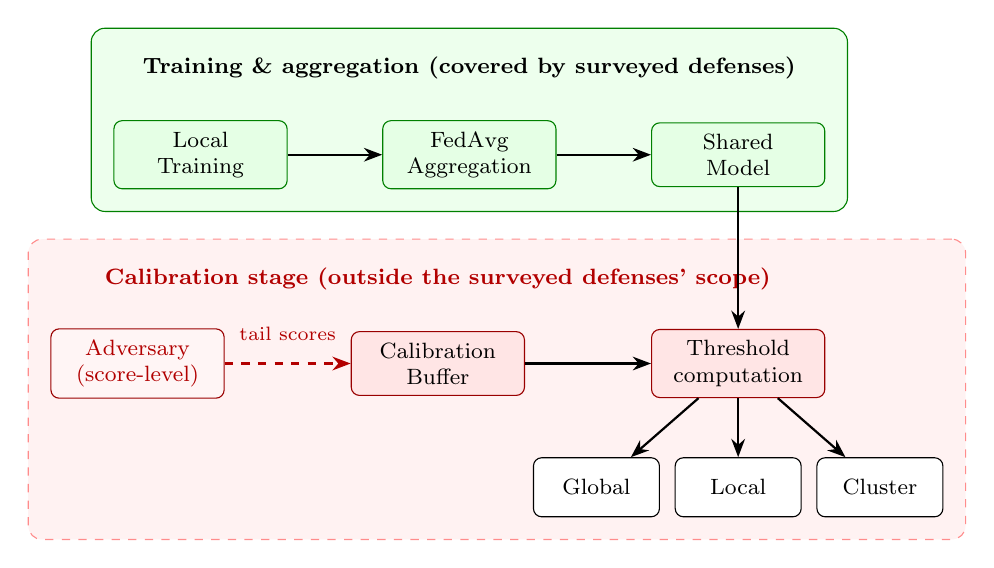
\begin{tikzpicture}[
  font=\footnotesize,
  box/.style={draw, rounded corners=3pt, minimum width=2.20cm, minimum height=0.75cm,
              align=center, fill=white, inner xsep=6pt, inner ysep=4pt},
  secure/.style={box, fill=green!10, draw=green!50!black},
  vuln/.style={box, fill=red!10, draw=red!60!black},
  attack/.style={box, fill=red!4, draw=red!60!black, text=red!70!black,
                 minimum width=2.20cm},
  policy/.style={box, minimum width=1.60cm},
  phaseLabel/.style={font=\footnotesize\bfseries, align=center, inner sep=2pt},
  arr/.style={-Stealth, thick},
  darr/.style={-Stealth, thick, red!70!black, dashed}
]
  \node[secure] (local) {Local\\Training};
  \node[secure, right=1.20cm of local] (agg)   {FedAvg\\Aggregation};
  \node[secure, right=1.20cm of agg]   (model) {Shared\\Model};
  \node[phaseLabel, above=0.45cm of agg] (trainLabel)
        {Training \& aggregation (covered by surveyed defenses)};

  \node[vuln,   below=1.80cm of model] (thresh) {Threshold\\computation};
  \node[vuln,   left=1.60cm of thresh] (cal)    {Calibration\\Buffer};
  \node[attack, left=1.60cm of cal]    (adv)    {Adversary\\(score-level)};
  \node[phaseLabel, text=red!70!black, above=0.45cm of cal] (calLabel)
        {Calibration stage (outside the surveyed defenses' scope)};

  \node[policy, below=0.75cm of thresh, xshift=-1.80cm] (pg) {\GLOBAL};
  \node[policy, below=0.75cm of thresh]                 (pl) {\LOCAL};
  \node[policy, below=0.75cm of thresh, xshift=+1.80cm] (pc) {\CLUSTER};

  \begin{scope}[on background layer]
    \node[draw=green!50!black, rounded corners=5pt, fill=green!7, inner sep=8pt,
          fit=(local)(agg)(model)(trainLabel)] {};
    \node[draw=red!45, rounded corners=5pt, fill=red!5, inner sep=8pt, dashed,
          fit=(calLabel)(adv)(cal)(thresh)(pg)(pl)(pc)] {};
  \end{scope}

  \draw[arr] (local) -- (agg);
  \draw[arr] (agg)   -- (model);
  \draw[arr] (model.south) -- (thresh.north);
  \draw[arr] (cal)   -- (thresh);
  \draw[arr] (thresh) -- (pg);
  \draw[arr] (thresh) -- (pl);
  \draw[arr] (thresh) -- (pc);
  \draw[darr] (adv) --
        node[midway, above=7pt, font=\scriptsize, red!70!black,
             fill=red!5, inner xsep=2pt, inner ysep=1pt]{tail scores} (cal);
\end{tikzpicture}%
}
\caption{Attack surface: threshold calibration occurs after FL training.
Green boxes mark training and aggregation; the dashed red region marks calibration, outside the scope of the defenses surveyed in Section~\ref{sec:background}.
The three policy nodes are alternative computations, not deployment components; score-level access to one client's calibration buffer can shift the resulting threshold(s) without modifying model weights, gradients, or labels.}
\label{fig:attack-surface}
\end{figure}

\section{Experimental Protocol}
\label{sec:method}

\subsection{Dataset and Federation}

The evaluation uses N-BaIoT~\cite{meidan2018nbaiot}, a labeled IoT traffic dataset covering nine physical devices across five types (doorbell, baby monitor, security camera, thermostat, webcam), each device forming one federation client; all nine satisfy the $\ge$100-sample calibration eligibility threshold (size range in Table~\ref{tab:repro}).
Each device's benign stream is partitioned chronologically into a $60\%$ train / $1\%$ gap / $20\%$ calibration / $1\%$ gap / $18\%$ test split, the gaps avoiding temporal leakage, and training and calibration use benign traffic only.
Attack-labeled records are scaled with each device's training-fitted scaler and used only as the positive class for TPR; they never enter training, calibration, poisoning reservoirs, or injected buffers.
The federation trains a shared autoencoder on benign traffic using FedAvg~\cite{mcmahan2017fedavg} (Table~\ref{tab:repro}); each client then scores its own traffic with the aggregated model and enters the threshold-calibration stage at $q{=}0.95$.

\begin{table}[tb]
\caption{Experimental configuration: architecture, federated training hyperparameters, and calibration settings.}
\label{tab:repro}
\centering
\footnotesize
\begin{tabular}{@{}ll@{}}
\toprule
Component & Configuration \\
\midrule
\multicolumn{2}{@{}l}{\emph{Autoencoder architecture}} \\
Input features & 115 (N-BaIoT statistical traffic features) \\
Encoder layers & $115 \to 80 \to 40 \to 20$; decoder mirrors \\
Activation & ReLU (no batch normalization) \\
Loss & Mean squared reconstruction error \\
Optimizer & Adam, learning rate 0.001, weight decay 0 \\
\midrule
\multicolumn{2}{@{}l}{\emph{Federated training (FedAvg)}} \\
Local epochs & 1 \\
Aggregation & Sample-count-weighted mean \\
Rounds & 40 initial, 150 max (conv.: $\Delta$loss\,$\le$\,0.005 over 10) \\
Batch size & 256 \\
\midrule
\multicolumn{2}{@{}l}{\emph{Calibration (per-device sizes in released split manifest)}} \\
Benign samples / device & 2,622 (Ecobee) -- 35,048 (Philips) \\
Threshold quantile $q$ & 0.95 \\
\bottomrule
\end{tabular}
\end{table}

\subsection{Threshold Policies}

Three threshold-policy families are evaluated, covering the design points surveyed in Section~\ref{sec:background}.

\begin{description}
  \item[\GLOBAL.]
  \[
    \tau_i^{\mathrm{local}} = \operatorname{quantile}(\mathcal{C}_i,q),
    \qquad
    \tau^{\mathrm{global}} = \frac{1}{N}\sum_{i=1}^{N}\tau_i^{\mathrm{local}} .
  \]
  Every client receives the same $\tau^{\mathrm{global}}$, so a single poisoned local threshold contributes only $1/N$ of the shared shift.

  \item[\LOCAL.] Each client retains $\tau_i = \tau_i^{\mathrm{local}}$.
  Shifts are confined to the compromised client; no cross-client threshold propagation.

  \item[\CLUSTER.]
  Clients are grouped on a standard-scaled 4-feature fingerprint (mean, std, skew, $p_{95}$ of $\mathcal{C}_i$) via $k$-means++~\cite{arthur2007kmeanspp} ($K{=}3$, 10 initializations, random seed 42; clustering recomputed after each attack draw).
  The shared threshold is the cluster mean, so a compromised client may perturb the threshold for co-cluster members (\emph{intra-cluster threshold perturbation}) while other clusters are unaffected.
  Recomputed assignments can also move non-victims, so even the direction of their threshold changes need not match the victim's.
\end{description}

\subsection{Attack Parameterization}

For each (policy, source--objective pair, injection fraction $f \in \{0,0.1,0.2,0.4\}$) combination the protocol runs 20 training seeds, each with a paired poisoning draw. A clean calibration array is preserved and only its poisoned copy enters threshold computation.
Six source--objective pairs are evaluated: High-Score-Benign with Threshold-Raise; Low-Score-Benign with Threshold-Lower; their objective-matched Random-Benign controls; and High-Score-Train-Feature-Benign with Threshold-Raise and its Random-Train-Feature-Benign control. In the feature variant, the donor pool comprises benign training-feature rows from the other eight devices, scored by the fixed model. Selected donor rows are drawn without replacement, so this sensitivity assumes cross-device feature access beyond the primary single-client buffer permission. Every client is victim in turn, giving $6\times3\times4\times9\times20=12{,}960$ objective-labeled rows, including 9,720 with non-zero injection. Shared clean comparators and rows from one training seed are not independent evidence.
Training seed $i$ is combined with poisoning seed $i{+}100$ and analysis seed $i{+}300$, separating training, poisoning draws, and resampling stochasticity.

\subsection{Statistical Analysis}

Clean and poisoned conditions are paired: for a policy, victim $v$, and seed $s$, the clean comparator is the $f{=}0$ cell produced by the same trained model and the same calibration array before replacement, so every reported difference is within-seed and within-victim,
\[
  \Delta\tau_{v,s} \;=\; \tau^{\mathrm{poisoned}}_{v,s} - \tau^{\mathrm{clean}}_{v,s},
\]
and likewise for $\Delta\mathrm{TPR}$ and $\Delta\mathrm{CV(FPR)}$.
The nine victim values within a seed are averaged into one seed-level aggregate, and the 20 paired aggregates are the inferential units: bootstrap resampling is over seeds, never over the 180 victim--seed cells, which share a trained model within a seed.
Three gates, all fixed before any poisoned run, structure the claims below.

\textbf{Gate 1 (material shift, primary gate)} evaluates the signed displacement $\Delta\tau_{v,s}$ at the victim--seed cell.
A cell is \emph{material} when $|\Delta\tau_{v,s}| \ge \delta\tau_{v,s}$ and its sign matches the objective---positive for raising, negative for lowering---so displacement in the wrong direction never counts, where
\[
  \delta\tau_{v,s} = \max\!\bigl(0.1\,b_{v,s},\;
  0.01\,\mathrm{median}_j(\mathrm{IQR}(\mathcal{C}_{j,s}^{\mathrm{clean}}))\bigr)
\]
is computed from the same seed's clean calibration arrays with $j$ over all nine clients. Here $b_{v,s}$ is the victim's clean IQR when positive, otherwise its median absolute deviation or, if needed, the minimum positive gap between distinct scores.
A \emph{seed passes} when at least 5 of the 9 clients, each taken as victim in turn, are material. A (policy, fraction, source) configuration passes Gate 1 when at least 16 of 20 seeds have the objective-aligned mean shift and meet this victim-majority criterion. These are operational consistency requirements, not calibrated error rates.
Passing describes material, directionally consistent displacement under these cutoffs; failure does not establish a null effect.
The 10\% IQR term and 1\% cross-client floor set a materiality scale; sensitivity to these choices is reported below.
Gate 1 is a materiality rule rather than a significance test; its seed pass counts appear in Table~\ref{tab:main-results}.

\textbf{Gate 2 (directional excess over control)} is an objective-matched paired contrast: within each cell the control $\Delta\tau$ is subtracted from the attack $\Delta\tau$, sign-oriented by objective, and the nine victim values are averaged to one value per seed.
A configuration passes when at least 16 of 20 seed values are strictly positive and their median is positive. A paired percentile bootstrap CI is reported separately and does not enter the rule.

\textbf{Gate 3 (downstream operating-point displacement)} passes if at least one prespecified downstream metric has 16/20 seed aggregates in the harmful direction and a positive median after sign orientation. For raising, these are mean victim TPR, balanced-accuracy, or macro-F1 loss, or the worst victim TPR loss within each seed. For lowering, they are increases in fleet mean FPR, CV(FPR), IQR(FPR), FPR range, or worst-client FPR. The victim TPR-loss and fleet mean-FPR counts are reported below as direct witnesses of the gate.
For raising, the threshold increase means reduced victim TPR and hence missed-detection harm.
For lowering, the threshold decrease raises false-positive burden and may change FPR disparity in either direction. The accompanying positive $\Delta\mathrm{TPR}$ indicates operating-point displacement, not a security benefit.

All CIs are 95\% percentile bootstrap over 20 seed-level aggregates with $B{=}10{,}000$ resamples, two-sided and without multiplicity adjustment. They are approximate uncertainty estimates. Exact sign-flip and binomial support diagnostics are available in the reporting artifacts; victim rows do not enlarge the inferential sample.

\subsection{Isolation Sanity Check}

To confirm that the attack is confined to calibration, the protocol verifies invariant AUROC and clean score ranks and bitwise-identical model weights; these checks hold throughout the completed main matrix, including 9,720 non-zero rows.
Being invariant by construction, these quantities verify implementation isolation rather than provide independent evidence.


\section{Results}
\label{sec:results}

\subsection{Clean policies and score scales}
The 20-seed clean profile (Table~\ref{tab:baseline}) shows the lowest FPR dispersion under \LOCAL and the highest under \GLOBAL. The paired seed-level Global--Local CV(FPR) difference is 0.595 [0.563, 0.628]; Global--Cluster is 0.297 [0.241, 0.346], and Cluster--Local is 0.298 [0.239, 0.366]. These differences do not establish an overall policy ranking: the P10 client Macro-F1 is 0.398 under \GLOBAL and 0.361 under \LOCAL. Figure~\ref{fig:clean-fpr} illustrates client FPRs in the seed selected by the lower-median Global CV(FPR) among the 20 seeds.
\begin{figure}[tb]
\centering
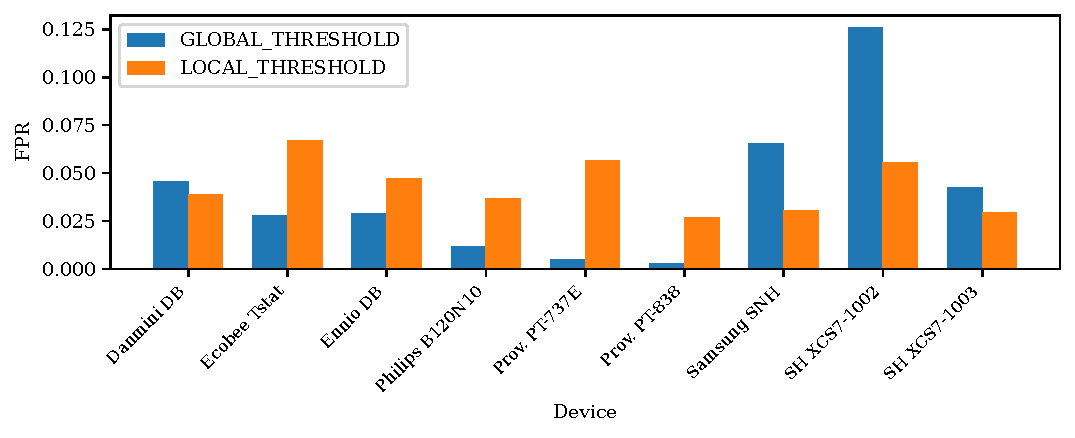
\includegraphics[width=0.95\textwidth]{figures/fig_clean_fpr.pdf}
\caption{Clean per-client FPR under \GLOBAL and \LOCAL for seed 4, selected as the lower-median Global CV(FPR) among all 20 seeds using clean metrics only. All-seed estimates appear in Table~\ref{tab:baseline}.}
\label{fig:clean-fpr}
\end{figure}
\begin{table}[tb]
\caption{Clean N-BaIoT baseline, 20 training seeds and nine clients. Dispersion and detection values are seed mean $\pm$ SD; FPR is the client/seed mean. CV is population SD / mean across clients; worst BA is the minimum per-client balanced accuracy; P10 Macro-F1 is the 10th percentile of per-client mean benign-class and attack-class F1.}
\label{tab:baseline}
\centering\scriptsize
\setlength{\tabcolsep}{2pt}
\begin{tabular}{@{}lccccc@{}}
\toprule
Policy & CV(FPR) & CV(TPR) & Worst BA & P10 F1 & FPR\\
\midrule
\GLOBAL & .919$\pm$.029 & .255$\pm$.024 & .658$\pm$.007 & .398$\pm$.052 & .04112\\
\LOCAL & .324$\pm$.058 & .280$\pm$.067 & .673$\pm$.059 & .361$\pm$.135 & .04346\\
\CLUSTER & .622$\pm$.128 & .295$\pm$.030 & .657$\pm$.004 & .322$\pm$.046 & .04404\\
\bottomrule
\end{tabular}
\end{table}


Raw local thresholds differ by a mean max/min ratio of 6.85 across devices; their mean cross-client CV is 0.655. The main \GLOBAL policy deploys one identical raw mean threshold to every client, although their score scales are heterogeneous. A scale-normalized Global consensus sensitivity divides each local threshold by that client's clean calibration median, averages the ratios, and back-transforms the mean with each client's median to obtain client-specific deployed thresholds. The clean medians remain frozen under poisoning; test scores and all other evaluation conditions are paired. At $f{=}0.4$ under raising, raw versus normalized victim $\Delta\mathrm{FPR}$ is $-0.00642$ versus $-0.00406$, and clean CV(FPR) is 0.919 versus 1.052. These are different deployment policies; neither is universally better on these metrics.

\subsection{Threshold displacement and matched controls}
Table~\ref{tab:main-results} reports all non-zero policy--fraction cells for the two within-calibration-tail attacks. Gate 2 is the objective-oriented, within-victim-and-seed attack-minus-matched-Random-Benign contrast, with a paired bootstrap interval; controls are never pooled across objectives. Every contrast is positive in 20/20 seed aggregates. Gate 3 passes in all 18 cells: victim TPR loss has 20/20 expected-sign seeds for every raising policy and fraction; for lowering, fleet mean absolute FPR increase has 20/20 for Global and Local at each fraction and 17/20, 17/20, and 18/20 for Cluster at $f{=}0.1,0.2,0.4$. All raising cells pass Gate 1. Lowering passes Gate 1 except Global at $f{=}0.1$, where only 4/20 seeds meet its victim-majority materiality rule. The Gate 3 fleet-FPR witness measures absolute burden, not FPR disparity. These gates measure consistency and materiality, not calibrated significance.
\begin{table}[tb]
\caption{20-seed main results. Raise/Lower use the original within-calibration tail. $\Delta\tau$ is a signed seed mean; Gate 2 is the positive, objective-oriented contrast against the objective-matched Random-Benign control [paired 95\% CI]. TPR is victim change in percentage points. G1 is the seed pass count; G2 is 20/20 for every row.}
\label{tab:main-results}
\centering\scriptsize
\setlength{\tabcolsep}{3pt}
\begin{tabular}{@{}llrrrrr@{}}
\toprule
Policy & Objective & $f$ & $\Delta\tau$ & Gate 2 [95\% CI] & G1 & $\Delta$TPR (pp)\\
\midrule
\GLOBAL & Raise & .1 & +.034 & .034 [.033,.036] & 20/20 & -4.5\\
 & & .2 & +.063 & .063 [.061,.065] & 20/20 & -5.1\\
 & & .4 & +.104 & .104 [.101,.107] & 20/20 & -6.6\\
\LOCAL & Raise & .1 & +.308 & .310 [.298,.323] & 20/20 & -6.5\\
 & & .2 & +.567 & .563 [.547,.581] & 20/20 & -7.3\\
 & & .4 & +.934 & .934 [.905,.964] & 20/20 & -7.9\\
\CLUSTER & Raise & .1 & +.260 & .261 [.238,.282] & 20/20 & -3.9\\
 & & .2 & +.524 & .527 [.507,.547] & 20/20 & -4.7\\
 & & .4 & +.930 & .931 [.897,.967] & 20/20 & -5.5\\
\midrule
\GLOBAL & Lower & .1 & -.006 & .006 [.005,.006] & 4/20 & +0.1\\
 & & .2 & -.011 & .012 [.011,.013] & 20/20 & +0.6\\
 & & .4 & -.019 & .018 [.017,.020] & 20/20 & +1.3\\
\LOCAL & Lower & .1 & -.056 & .054 [.049,.058] & 20/20 & +3.2\\
 & & .2 & -.099 & .106 [.098,.115] & 20/20 & +5.5\\
 & & .4 & -.169 & .166 [.155,.177] & 20/20 & +11.3\\
\CLUSTER & Lower & .1 & -.056 & .053 [.042,.066] & 20/20 & +3.5\\
 & & .2 & -.101 & .100 [.086,.114] & 20/20 & +5.2\\
 & & .4 & -.159 & .156 [.139,.171] & 20/20 & +9.4\\
\bottomrule
\end{tabular}
\end{table}


At $f{=}0.4$ raising, victim TPR changes by $-6.6$ pp under \GLOBAL, $-7.9$ pp under \LOCAL, and $-5.5$ pp under \CLUSTER. The corresponding 95\% seed-bootstrap intervals are $[-8.2,-4.9]$, $[-10.4,-5.9]$, and $[-7.3,-4.0]$ pp. The victim-level \LOCAL changes range from $-0.03$ pp for SimpleHome XCS7-1002 to $-19.5$ pp for Ennio; the mean does not describe every device. Exact paired decision-count differences average 29,507, 52,300, and 39,998 additional missed attack records per victim experiment, respectively, over device attack test sets of 316,400--968,750 records. The corresponding unweighted mean client-rate differences imply 662, 788, and 550 extra misses per 10,000 attack observations. Both summaries first average the nine victim experiments within each seed and then the 20 seeds; the standardized rates are not ratios of pooled counts. These test-set counts are not fixed-time deployment forecasts.
\begin{figure}[tb]
\centering
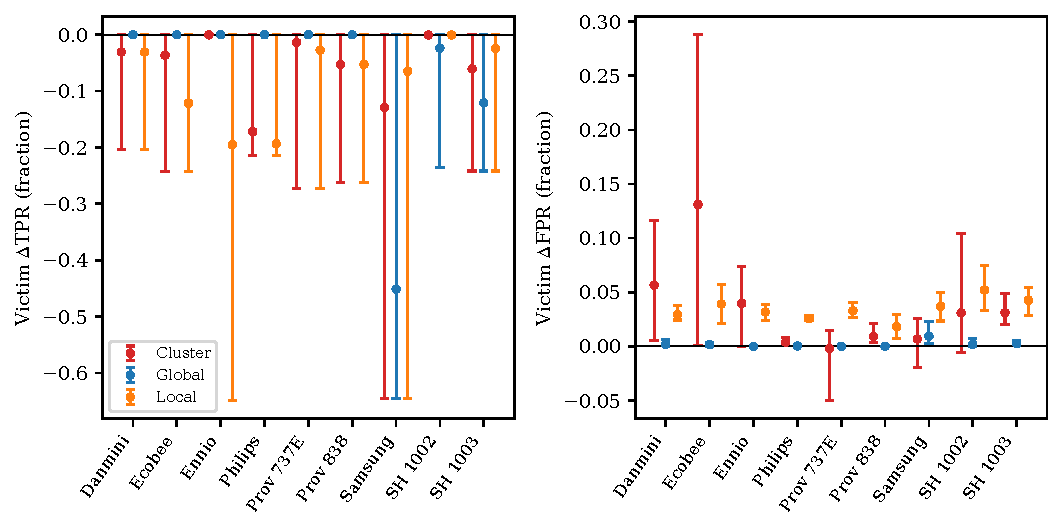
\includegraphics[width=\textwidth]{figures/fig_client_effects.pdf}
\caption{Victim-level raising $\Delta$TPR (left) and lowering $\Delta$FPR (right) at $f{=}0.4$ over 20 training seeds. Axes show fractional rate differences (multiply by 100 for percentage points); points show client means and bars show observed seed minima and maxima, not confidence intervals. Prov denotes Provision cameras; SH denotes SimpleHome cameras. Client variation is descriptive; the seed remains the independent inferential unit.}
\label{fig:client-effects}
\end{figure}

At $f{=}0.4$ lowering, victim $\Delta\mathrm{FPR}$ is $+0.00193$ [0.00165, 0.00224] for \GLOBAL, $+0.03433$ [0.03348, 0.03523] for \LOCAL, and $+0.03410$ [0.02989, 0.03826] for \CLUSTER. Fleet mean absolute FPR rises by 0.00171 [0.00156, 0.00188], 0.00381 [0.00372, 0.00391], and 0.00584 [0.00431, 0.00715], respectively. Fleet $\Delta\mathrm{CV(FPR)}$ is $-0.021$ [$-0.023,-0.019$], $+0.058$ [0.049, 0.067], and $+0.065$ [0.006, 0.116]. Lowering raises victim TPR through a lower decision boundary; it does not improve the security interpretation. Exact paired false-alarm count differences average 16, 335, and 199 per victim experiment, respectively, over device benign test sets of 2,362--31,544 records. The unweighted mean client-rate differences correspond to 19, 343, and 341 additional false alarms per 10,000 benign observations. Counts and rates are averaged over nine victims within each of 20 seeds as above.

\subsection{Non-victim propagation and cluster stability}
Under raising at $f{=}0.4$, mean non-victim TPR change is $-3.93$ pp [$-4.96,-2.91$] for \GLOBAL, zero for \LOCAL, and $+1.55$ pp [0.29, 2.89] for recomputed \CLUSTER. Mean non-victim $\Delta\mathrm{FPR}$ is $-0.00643$ [$-0.00697,-0.00592$] for Global and $-0.00011$ [$-0.00214,0.00159$] for Cluster. The Cluster mean conceals assignment-driven gains and losses. Under lowering, non-victim mean $\Delta\mathrm{FPR}$ is $+0.00168$ [0.00154, 0.00184] for Global and $+0.00231$ [0.00077, 0.00358] for Cluster; Local is zero by construction. The corresponding non-victim $\Delta\mathrm{TPR}$ values are $+0.73$ pp [0.35, 1.14] and $+0.63$ pp [$-0.16$, 1.50], respectively; this is the expected tradeoff from a lower threshold, and Cluster's interval includes zero. Global adds a mean 112 false positives across eight non-victims per victim experiment on their full benign test sets.

For \CLUSTER raising at $f{=}0.4$, 86.7\% of the 180 victim--seed evaluations change the partition; on average, 7.3 of nine clients change their set of cluster co-members. This label-invariant count includes clients affected by another client's move; it is not a count of raw K-means label mismatches. The victim is a singleton in 48.9\% of poisoned evaluations, versus none of the clean ones. Modal cluster sizes remain [4,3,2], and mean victim cluster size changes from 3.21 to 2.48. Holding clean assignments fixed reduces mean victim $\Delta\tau$ from 0.930 to 0.333 and changes mean non-victim $\Delta\mathrm{TPR}$ from $+1.55$ to $-0.83$ pp. Recomputed Cluster behavior is therefore sensitive to assignment changes. In the $K\in\{2,3,4\}$ and $n_{\rm init}\in\{1,10\}$ grid, the $K{=}3$, $f{=}0.4$ raising mean shift is 0.853 for one initialization and 0.930 for ten.

\subsection{Intervention and gate sensitivity}
The separate cross-device benign training-feature reservoir is scored with the fixed model and sampled without repeating donor feature rows. At $f{=}0.4$ its high-score raising variant yields mean victim $\Delta\tau$ of 0.024 (Global), 0.214 (Local), and 0.166 (Cluster), below same-calibration-tail values of 0.104, 0.934, and 0.930. Global at $f{=}0.1$ does not pass Gate 1 for this variant. It demonstrates a distinct, score-generating feature source under broader donor access, though not an adversary's ability to obtain or produce those features as traffic. Under the original same-buffer draw, mean duplicate rate at Local $f{=}0.4$ is 0.366 versus 0.012 for an interpolated-tail sensitivity variant, whose mean threshold shift is 0.932 versus 0.934. Interpolation synthesizes scores rather than traffic. Without-replacement and disjoint-tail variants cannot meet the full 40\% budget with the 10\% tail; reduced-budget effects cannot be compared as equal-dose attacks.

The prespecified gate uses 5/9 victims and 16/20 seeds. The 225-point Cartesian sensitivity grid varies seed support from 12 to 20, victim majority from 3 to 7, the IQR materiality factor from 0.05 to 0.20, and the cross-client IQR floor from 0.005 to 0.020. All three main $f{=}0.4$ raising cells retain Gates 1--3 across the grid; Global and Cluster retain the full-vulnerability classification in 225/225 settings, while Local does so in 219/225 because the control-instability classification changes. Lowering classifications are less stable: Global at $f{=}0.1,0.2,0.4$ differs from baseline in 78, 99, and 45 settings; Cluster at those fractions in 123, 27, and 48, with Gate 3 changing in 90 settings at $f{=}0.1$ and 45 at $f{=}0.4$. Local lowering at $f{=}0.1$ changes in 21 settings, while $f{=}0.2,0.4$ remain stable. Most other main-matrix changes arise from Gate 1 materiality/support or control-instability criteria; the separate feature-reservoir variant is also cutoff-sensitive. Thus the gate classification is conditional on its operational cutoffs; effect sizes and paired intervals remain the quantitative evidence.


\section{Discussion and Limitations}
\label{sec:discussion}

The main experiment substitutes reconstruction scores directly. It demonstrates sensitivity of the threshold computation to a writable calibration input, not the ability to generate IoT packets that produce the selected scores. The separate cross-device training-feature reservoir shows that model-scored benign feature rows outside the calibration split can supply effective donors; their availability or controllability by a real adversary is untested. The experimental trust boundary also assumes that the threshold code and final threshold cannot be overwritten directly while the input buffer can. A deployment would require explicit enforcement of that boundary.

With-replacement sampling from the same calibration tail reweights observed values and introduces detectable duplicates. The interpolated-score sensitivity preserves much of the measured displacement while reducing exact duplication, but it still does not establish traffic feasibility. The lowering attack uses random replacement positions; its effects should not be interpreted as the largest achievable under a rank-aware adversary.

Policy effects have different failure modes. \LOCAL confines the attack to its victim, whose detection loss can be large. \GLOBAL dilutes one local-threshold shift by $1/9$ yet changes all clients' operating points; its raw thresholds arise from heterogeneous client scales. \CLUSTER has assignment-dependent victim and non-victim effects, including opposite signs across clients. Fixed-assignment and $K$/initialization sensitivities limit any general claim that clustering reliably isolates contamination. The gate thresholds were chosen as consistency and materiality criteria, and sensitivity analyses show that gate decisions depend on those choices; percentile intervals at 20 seeds remain approximate.

The scope is one dataset, nine devices, a FedAvg autoencoder, $q{=}0.95$, and one compromised client at a time. Neither multi-client collusion nor calibration-input integrity mechanisms were evaluated. These limits constrain deployment claims while leaving the controlled score-level result intact.


\section{Conclusion}
\label{sec:conclusion}

In a 20-seed, nine-device N-BaIoT evaluation, poisoning one client's post-training calibration scores shifted thresholds and detection outcomes without changing model weights or test scores. Raising with same-buffer high-tail scores met the materiality rule under all three policies and all non-zero fractions; at 40\% replacement, victim TPR fell by 5.5--7.9 percentage points. Global spread a smaller threshold shift to all clients and lowered mean non-victim TPR by 3.93 points, Local isolated non-victims, and recomputed Cluster showed assignment-sensitive effects. Lowering raised absolute FPR burden even where FPR dispersion decreased. A separate benign feature reservoir yielded smaller but directional shifts. These findings characterize a score-level calibration vulnerability and motivate protecting calibration inputs and threshold computation; traffic-level realizability and generalization to other systems remain to be tested.

\textbf{Reproducibility.}
The project artifact records configuration, paired training/poisoning/analysis seeds, per-client results, controls, sensitivity analyses, and reporting scripts. The conclusions here use the completed 20-seed campaign.


\begin{credits}
\subsubsection{\discintname}
The authors have no competing interests to declare that are relevant to the content of this article.
\end{credits}

\bibliographystyle{splncs04}
\bibliography{references}

\end{document}
